% !TEX root = review.tex

\subsection{Pure iron phase diagram}
\label{ssec:phase}

The earth has a solid inner core and liquid outer core.
The composition of the cores is still not very clear until now.
Over $90\%$ of it is made of \ce{Fe},
and opinions are divided on the rest parts.
From a cosmochemical and geochemical view,
the rest part consists of up to $10\%$ of \ce{Ni}\cite{McDonough:1995iz}.
But this fails to explain the core's
density, seismic wave velocities
and seismic anisotropy.
From a seismological view, the core contains
$2-3\%$ of light elements, like \ce{S}, \ce{O}, \ce{Si}, \ce{H} and \ce{C}, etc.
Especially the inner core,
according to seismological models, it is anisotropic, layered, and laterally heterogeneous, but the origins are not fully understood.
Besides,
at the inner-core-boundary (ICB),
the temperature must be the liquidus temperature of what the core is made of.
Thus \ce{Fe}'s melting temperature at the pressure of
the ICB will give a close estimation.
So to study iron's behavior under extreme high pressure and temperature
conditions is of great importance in understanding the earth's core.
That is to say, we need a complete phase diagram of \ce{Fe}, with
$T$ and $P$ as horizontal and vertical axes.

\begin{figure}[h]
	\centering
	\begin{minipage}[t]{.5\linewidth}
		\centering
		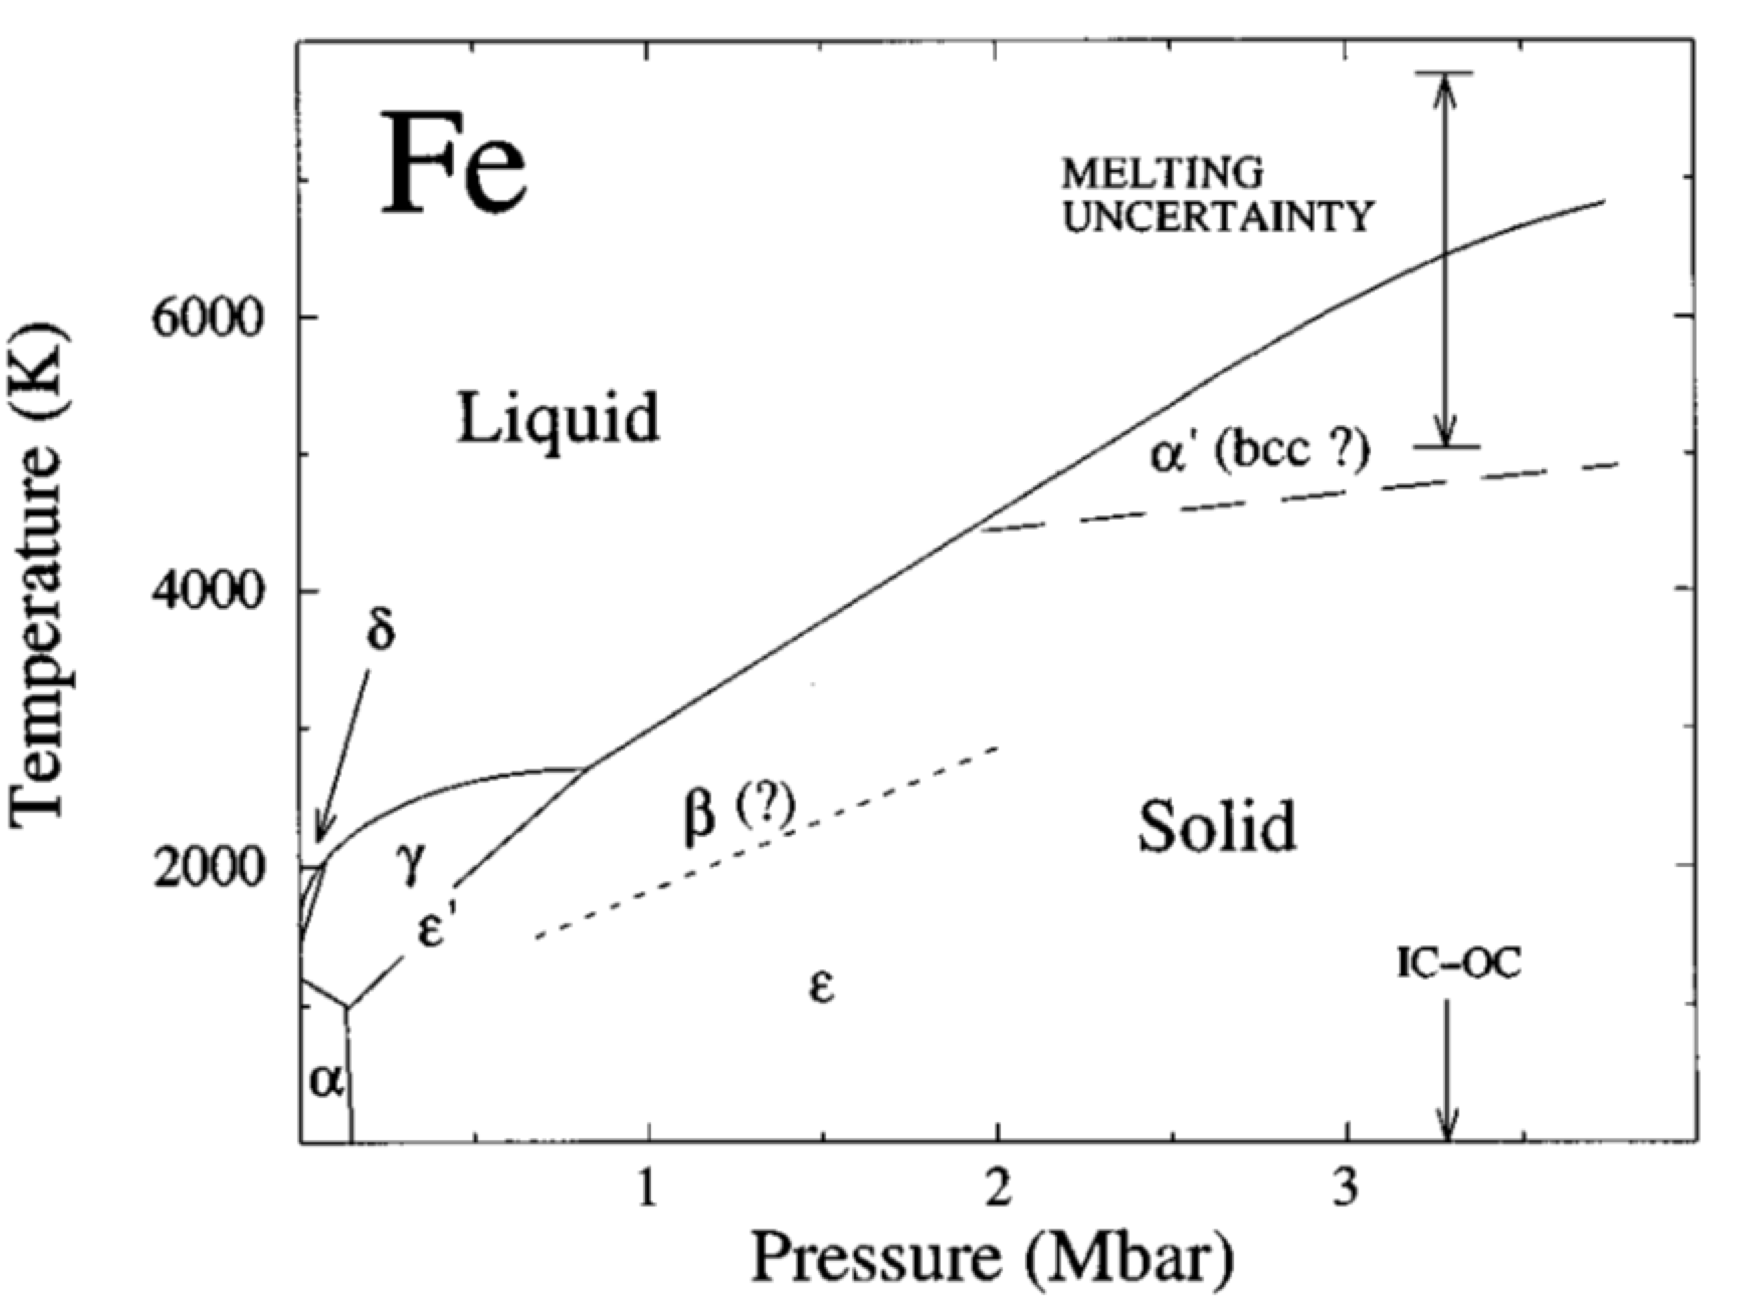
\includegraphics[width=\linewidth]{s1996}
		\caption{Possible high-pressure phase diagram of Fe, including established phases    bcc, fcc, bcc, and hcp as well as proposed some phases dhcp and unknown up to
			1996\cite{Soderlind:1996du}.}
		\label{fig:fepd:a}
	\end{minipage}%
	\hfil
	\begin{minipage}[t]{.5\linewidth}
		\centering
		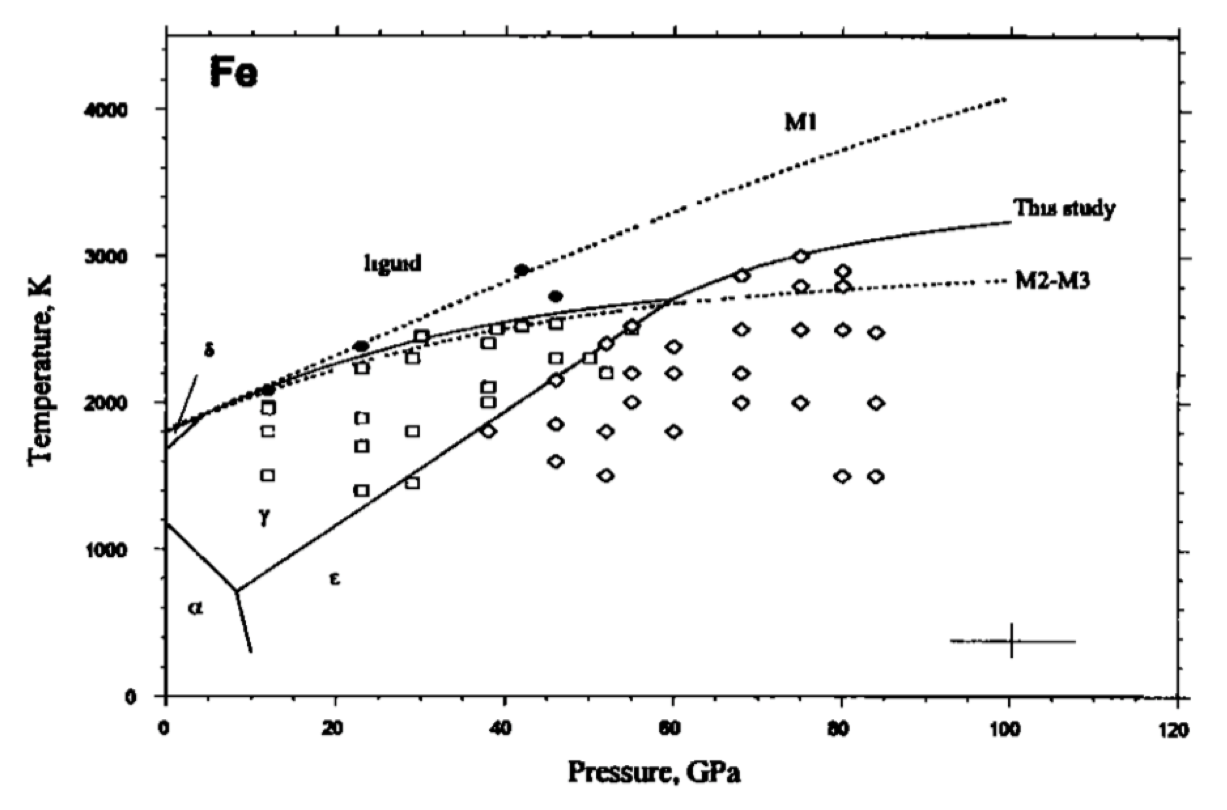
\includegraphics[width=\linewidth]{shen1998}
		\caption{Shen \textit{et. al.}\cite{Shen:1998bt}
			improved their laser-heated DAC to give a
			more precise phase diagram for \ce{Fe} at low pressure-temperature range.}
		\label{fig:fepd:b}
	\end{minipage}
\end{figure}

From Fig. \ref{fig:fepd:a} we can see that a collection of found phases up
till 1996.
$\alpha$- and $\delta$-phase are both hcp phases, $\gamma$-phase
is a fcc phase, and $\varepsilon$-phase is what we will mainly
talk about---hcp phase.
Near the boundary between $\gamma$ and $\varepsilon$ phase,
there was an assumed $\varepsilon'$---double hcp (dhcp) phase.
And they also suppose there should be an orthorhombic $\beta$-phase.
However, later Shen \textit{et. al.}\cite{Shen:1998bt} found that the appearance of the
dhcp structure is an effect of the temperature gradient in earlier experiments,
that is, an incomplete transition between $\varepsilon$ and $\gamma$.
They also concluded there are no stability fields for $\beta$ and $\varepsilon'$ phases.
See Fig.~\ref{fig:fepd:b} for reference.
There were body-centered tetragonal phase proposed either, but then be argued not
to be real by Shen\cite{Shen:1998bt} and Yoo\cite{Yoo:1995kx}.








